\section{Introduction}

\textbf{\color{red}Submission rules}
\begin{itemize}
\color{red}
\item submission only in pdf format
\item two column format
\item font size 11 for main text, abstract and references can use font size 9 (footnotesize in Latex)
\item maximum 4 A4 pages including everything (strict limit)
\item In addition: prepare short abstract (max 150 words) to be entered in the online submission system. 
      This will only be used for the program. 
      It will not be used for the review process nor for the final proceedings.
\end{itemize}

\lipsum[2-5]


\section{Materials and Methods}

This is how you add one \cite{Pivot2023} or multiple citations \cite{Saporta2022,Robert2022}.

% example equation
And this is a dummy equation
\begin{equation}
I_\alpha = \int_0^\alpha f(x) dx
\end{equation}

% example two column figure (use figure instead of figure* for one column figure)
\begin{figure*}
  \centering
  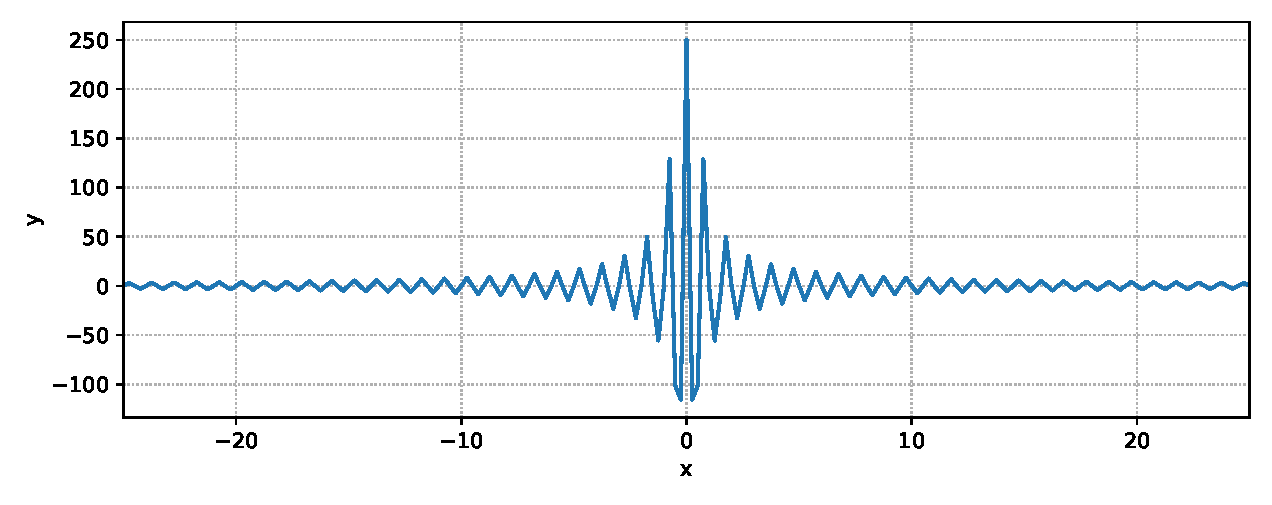
\includegraphics[width=1.0\textwidth]{./fig1.pdf}
  \caption{This a dummy figure to be replaced.}
  \label{fig:dummyfigure}
\end{figure*}

Figure \ref{fig:dummyfigure} shows how to include a figure.
Table \ref{tab:dummytable} shows how to include a table.

\bigskip

\lipsum[2-7]

\section{Results}
\subsection{Simulation results}

\lipsum[2-3]

\subsection{Other results}
\lipsum[2-3]

% example table
\begin{table}
  \centering
  \begin{tabular}{lrrr}
  \toprule
  $\alpha$   & $\beta$ & $\gamma$ & $\delta$ \\
  \midrule
  A          & 1       & a        & 3        \\
  B          & 2       & b        & 2        \\
  C          & 3       & c        & 1        \\
  \bottomrule
  \end{tabular}
  \caption{This is a dummy table to be replaced.}
  \label{tab:dummytable}
\end{table}



\section{Discussion}
\lipsum[2-9]


\section{Conclusion}
\lipsum[2]


